\begin{frame}
	\myheading{Module 8.2 : Train error vs Test error}
\end{frame}

\begin{frame}
	\begin{columns}
		\begin{column}{0.4\textwidth}
			\begin{itemize}
				\item<3-> We can show that
				\begin{align*}
					E[ (y-\hat{f}(x))^2 ] & = Bias^2					 &   \\
								    & +Variance					&   \\
								    & + \sigma^2 \text{ (irreducible error)} &   
				\end{align*}
								
				\item<4-> \href{http://www.inf.ed.ac.uk/teaching/courses/mlsc/Notes/Lecture4/BiasVariance.pdf}{\textcolor{blue}{See proof here}}
			\end{itemize}
							
		\end{column}
		\begin{column}{0.55\textwidth}
			\begin{itemize}
				\justifying
				\setlength\itemsep{1em}
				\item<1-> Consider a new point $(x,y)$ which was not seen during training
				\item<2-> If we use the model $\hat{f}(x)$ to predict the value of $y$ then the mean square error is given by
									
				\begin{align*}
					E[(y-\hat{f}(x))^2] 
				\end{align*}
				(average square error in predicting $y$ for many such unseen points)
								
			\end{itemize}
		\end{column}
	\end{columns}
\end{frame}
%%%%%%%%%%%%%%%%%%%%%%%%%%%%%%%%%%%%%%%%%%%%%%%%%%%%%%%%%%%%%
\begin{frame}
	\begin{columns}
		\begin{column}{0.4\textwidth}
			\onslide<4->{
				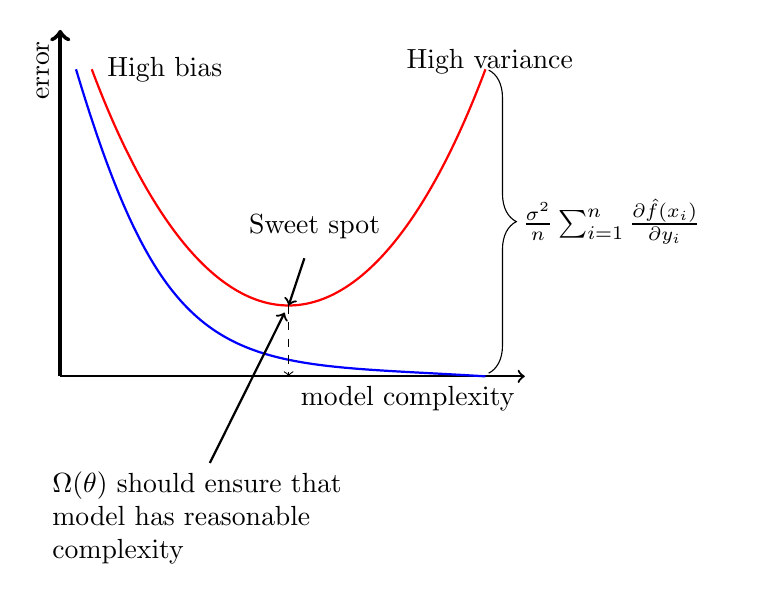
\begin{tikzpicture}
	\draw[->,thick] (4.1,-0.9)--(10,-0.9) node[below left]{model complexity};
	\draw[->,ultra thick] (4.1,-0.9)--(4.1	,3.5) node[above left,rotate=90]{error};
				
	\draw[red,thick] (4.5,3) .. controls (6,-1) and (8,-1) .. (9.5,3);
	\draw[blue,thick] (4.3,3) .. controls (5.5,-1) and (6.3,-0.7) .. (9.5,-0.9);
	\node[text width=4cm] at (6.7,3) {High bias};
	\node[text width=4cm] at (10.5,3.1) {High variance};
	\node[text width=3cm] at (8,1) {Sweet spot};
	\draw[->,thick] (7.2,0.6)--(7,0);	
	\draw[->,dashed] (7,0)--(7,-0.9);
	\draw[->,thick] (6,-2) -- (6.95,-0.09);	
	\node[text width=4cm] at (6,-2.7) {$\Omega(\theta)$ should ensure that model has reasonable complexity};
				
	%
	\draw [decorate,decoration={brace,amplitude=10pt,mirror,raise=4pt},yshift=0pt]
	(9.4,-0.86) -- (9.4,2.99) node [black,midway,xshift=1.7cm] {
		$\frac{\sigma^2}{n}\sum_{i=1}^{n}\frac{\partial\hat{f}(x_i)}{\partial y_i}$};	
\end{tikzpicture}
			}
			
			\onslide<10->{	\begin{align*}
				E[ (y-\hat{f}(x))^2 ] &= Bias^2&\\
				&+Variance&\\
				&+ \sigma^2 \text{ (irreducible error)}&
				\end{align*}}
		\end{column}
		\begin{column}{0.6\textwidth}
			\begin{itemize}
				\justifying
				\setlength\itemsep{1em}
				\item<1-> The parameters of $\hat{f}(x)$ (all $w_i$'s) are trained using a training set $\{(x_i,y_i)\}_{i=1}^{n}$
				\item<2-> However, at test time we are interested in evaluating the model on a validation (unseen) set which was not used for training
										
				\item<3-> This gives rise to the following two entities of interest:\\
				\color{blue}	$train_{err}$	(say, mean square error)\\
				\color{red} $test_{err}$ (say, mean square error)
										
				\item<4-> Typically these errors exhibit the trend shown in the adjacent figure
			\end{itemize}
		\end{column}
	\end{columns}
\end{frame}
%%%%%%%%%%%%%%%%%%%%%%%%%%%%%%%%%%%%%%%%%%%%%%%
\begin{frame}{}
	\begin{block}{Intuitions developed so far}
					
					
		\begin{itemize}
			\justifying
			\setlength\itemsep{1em}
			\item<1-> Let there be $n$ training points and $m$ test (validation) points	
			\begin{align*}
				train_{err} & = \frac{1}{n}\sum_{i=1}^{n}(y_i-\hat{f}(x_i))^2   &   \\
				test_{err}  & = \frac{1}{m}\sum_{i=n+1}^{n+m}(y_i-\hat{f}(x_i)) &   
			\end{align*}
			\item<2-> As the model complexity increases $train_{err}$ becomes overly optimistic and gives us a wrong picture of how close $\hat{f}$ is to $f$
			\item<3-> The validation error gives the real picture of how close $\hat{f}$ is to $f$
			\item<4-> We will concretize this intuition mathematically now and eventually show how to account for the optimism in the training error
		\end{itemize}			
	\end{block}
\end{frame}
%%%%%%%%%%%%%%%%%%%%%%%%%%%%%%%%%%%%%%%%%%%%%%%%
\begin{frame}
	\begin{columns}
		\begin{column}{0.5\textwidth}
			\begin{itemize}\justifying
				\setlength\itemsep{1em}
				\item<1-> Let D=$\{x_i,y_i\}_{i=1}^{m+n}$, then for any point $(x,y)$ we have,
				\begin{align*}
					y_i=f(x_i)+\varepsilon_i
				\end{align*}
				\item<2->which means that $y_i$ is related to $x_i$ by some true function $f$ but there is also some noise $\varepsilon$ in the relation
				\item<3->For simplicity, we assume 
				\begin{align*}
					\varepsilon\sim\mathcal{N}(0,\sigma^2)
				\end{align*}
				\onslide<4->{and of course we do not know $f$}
			\end{itemize}
		\end{column}
		\begin{column}{0.5\textwidth}
			\begin{itemize}\justifying
				\item<5-> Further we use $\hat{f}$ to approximate $f$ and estimate the parameters using T $\subset$ D such that
				\begin{align*}
					y_i=\hat{f}(x_i)
				\end{align*}
				\item<6-> We are interested in knowing 
				\begin{align*}
				E[(\hat{f}(x_i)-f(x_i))^2] 
				\end{align*}
				\onslide<7->{but we cannot estimate this directly because we do not know $f$}
				\item<8-> We will see how to estimate this empirically using the observation $y_i$ \& prediction $\hat{y}_i$
									
			\end{itemize}
		\end{column}
	\end{columns}
\end{frame}


%%%%%%%%%%%%%%%%%%%%%%%%%%%%%%%%%%%%%%%%%%%%%%%%%%%%%%%%%%%%%%%%%%%%%%%%
\begin{frame}
						
					
	\begin{align*}
		E[(\hat{y_i}   -y_i)^2] &
		\onslide<2->{  =E[(\hat{f}(x_i)-f(x_i)-\varepsilon_i)^2] \quad \textcolor{red}{(y_i=f(x_i)+ \varepsilon_i)}}													     \\\\
		\onslide<3->{ & =E[(\hat{f}(x_i)-f(x_i))^2-2\varepsilon_i(\hat{f}(x_i)-f(x_i))+\varepsilon_i^2]}																\\\\
		\onslide<4->{ & =E[(\hat{f}(x_i)-f(x_i))^2]-2E[\varepsilon_i(\hat{f}(x_i)-f(x_i))]+E[\varepsilon_i^2]}															\\\\
		% \only<4>{     & =E[(\hat{f}(x_i)-f(x_i))^2]-2E[(y_i-f(x_i))(\hat{f}(x_i)-f(x_i))]+E[\varepsilon_i^2] \quad \textcolor{red}{(\varepsilon_i = y_i - f(x_i))}}						 
		% \onslide<5->{ & \msout{=E[(\hat{f}(x_i)-f(x_i))^2]-2E[(y_i-f(x_i))(\hat{f}(x_i)-f(x_i))]+E[\varepsilon_i^2] \quad \textcolor{red}{(\varepsilon_i = y_i - f(x_i))}}}				     \\\\
		\onslide<5->{ \therefore E[(\hat{f}(x_i)-f(x_i))^2]\ & =\ E[(\hat{y_i}-y_i)^2]\ -\ E[\varepsilon_i^2]\ +\ 2E[\ \varepsilon_i(\hat{f}(x_i)-f(x_i))\ ]} 
	\end{align*}
					
\end{frame}
							
				
%%%%%%%%%%%%%%%%%%%%%%%%%%%%%%%%%%%%%%%%%%%%%%%%%%%%%%%%%%%
\begin{frame}
	\begin{block}{}
		We will take a small detour to understand how to empirically estimate an Expectation and then return to our derivation
	\end{block}
\end{frame}
%%%%%%%%%%%%%%%%%%%%%%%%%%%%%%%%%%%%%%%%%%%%%%%%%%%%%%%%%%%%
\begin{frame}
	\begin{itemize}
		\justifying
		\setlength\itemsep{1em}
		\item<1-> Suppose we have observed the goals scored($z$) in $k$ matches as \\$z_1=2$, $z_2=1$, $z_3=0$, ... $z_k=2$
		\item<2-> Now we can empirically estimate $E[z]$ i.e. the expected number of goals scored as
		\begin{align*}
			E[z]=\frac{1}{k}\sum_{i=1}^{k}z_i 
		\end{align*}
		\item<3-> Analogy with our derivation: We have a certain number of observations $y_i$ \& predictions $\hat{y_i}$ using which we can estimate
		\begin{align*}
			E[(\hat{y_i}-y_i)^2]= \onslide<4->{\frac{1}{m}\sum_{i=1}^{m}(\hat{y_i}-y_i)^2} 
		\end{align*}
	\end{itemize}
		
\end{frame}
%%%%%%%%%%%%%%%%%%%%%%%%%%%%%%%%%%%%%%%%%%%%%%%%%%%%%%%%%%%%%%
\begin{frame}
	\begin{block}{}
		... returning back to our derivation
	\end{block}
\end{frame}
%%%%%%%%%%%%%%%%%%%%%%%%%%%%%%%%%%%%%%%%%%%%%%%%%%%%%%%%%%%%%
\begin{frame}
						
					
	\onslide<1->	\begin{block}
	\
	%			\begin{align*}
	$E[(\hat{f}(x_i)-f(x_i))^2]\ =\ E[(\hat{y_i}-y_i)^2]\ -\ E[\varepsilon_i^2]\ +\ 2E[\ \varepsilon_i (\hat{f}(x_i)-f(x_i))\ ]$
	%\end{align*}		
	\end{block}
	\begin{itemize}
		\justifying
		\setlength\itemsep{1em}
		\item<2->	We can empirically evaluate R.H.S using training observations or test observations\linebreak\\\textbf{Case 1}: Using test observations
		\item[]<3-> 
			\scalebox{0.9}{\parbox{\linewidth}{%
				\begin{align*}
					\onslide<3->{ & \underbrace{	E[(\hat{f}(x_i)-f(x_i))^2]}_{true\hspace{0.05cm} error}}
					\onslide<4->{ & =\underbrace{\frac{1}{m}\sum_{i=n+1}^{n+m}(\hat{y_i}-y_i)^2}_{empirical\hspace{0.05cm}estimation\hspace{0.09cm}of\hspace{0.09cm}error}-} 
					\onslide<5->{\underbrace{\frac{1}{m}\sum_{i=n+1}^{n+m}\varepsilon_i^2}_{small\hspace{0.05cm}constant}} 
					\onslide<6->{+\ 2\underbrace{E[\ \varepsilon_i (\hat{f}(x_i)-f(x_i))\ ]}_{
					= \hspace{0.09cm}\textcolor{red}{covariance\hspace{0.05cm}(\varepsilon_i,\hat{f}(x_i)-f(x_i))}
					}}	
				\end{align*}
			}}
		\vspace{-10mm}
		\item[]<7-> 
			\begin{align*}
				\because \text{covariance}(X,Y) 
				\onslide<8-> {& = E[(X-\mu_X)(Y-\mu_Y)]\\}
				\onslide<9-> {& = E[(X)(Y-\mu_Y)] (\text{if } \mu_X=E[X]=0)\\} 
				\onslide<10-> {& = E[XY] - E[X\mu_Y]}
				\onslide<11-> {= E[XY] - \mu_Y E[X]}
				\onslide<12-> {= E[XY]}
			\end{align*}
	\end{itemize}
\end{frame}
			
%%%%%%%%%%%%%%%%%%%%%%%%%%%%%%%%%%%%%%%%%%%%%%%%%%%%%%%%%%%%%
\begin{frame}
	\onslide<1->\begin{align*}
	&\underbrace{	E[(\hat{f}(x_i)-f(x_i))^2]}_{true\hspace{0.09cm} error}\\&=\underbrace{\frac{1}{m}\sum_{i=n+1}^{n+m}(\hat{y_i}-y_i)^2}_{empirical\hspace{0.09cm}estimation\hspace{0.09cm}of\hspace{0.09cm}error}-\underbrace{\frac{1}{m}\sum_{i=n+1}^{n+m}\varepsilon_i^2}_{small\hspace{0.09cm}constant}\ +\ 2\underbrace{E[\ \varepsilon_i (\hat{f}(x_i)-f(x_i))\ ]}_{= \hspace{0.09cm}covariance\hspace{0.05cm}(\varepsilon_i,\hat{f}(x_i)-f(x_i))}
	\end{align*}
	\begin{itemize}
		\justifying
		\setlength\itemsep{1em}
		\item<2->None of the test observations participated in the estimation of $\hat{f}(x)$[the parameters of $\hat{f}$(x) were estimated only using training data]
		\begin{align*}
		\onslide<3->{&\therefore \varepsilon\perp (\hat{f}(x_i) - f(x_i)) }\\
		\onslide<4->{&\therefore E[\varepsilon_i \cdot ( \hat{f}(x_i)-f(x_i))]}
		\onslide<5->{=E[\varepsilon_i] \cdot E[\hat{f}(x_i)-f(x_i))]}
		\onslide<6->{=0 \cdot E[\hat{f}(x_i)-f(x_i))]}
		\onslide<7->{=0}\\
		\onslide<8->{&\therefore \text{true error = empirical test error + small constant}}
		\end{align*}
		\item<9-> Hence, we should always use a validation set(independent of the training set) to estimate the error
	\end{itemize}
\end{frame}			
%%%%%%%%%%%%%%%%%%%%%%%%%%%%%%%%%%%%%%%%%%%%%%%%%%%%%%%%%%%%
			
%%%%%%%%%%%%%%%%%%%%%%%%%%%%%%%%%%%%%%%%%%%%%%%%%%%%%%%%%
\begin{frame}
	\begin{itemize}
		\justifying
		\setlength\itemsep{1em}
		\item[]<1-> \textbf{Case 2}: Using training observations\begin{align*}
			&\underbrace{	E[(\hat{f}(x_i)-f(x_i))^2]}_{true\hspace{0.09cm} error}\\&=\underbrace{\frac{1}{n}\sum_{i=1}^{n}(\hat{y_i}-y_i)^2}_{empirical\hspace{0.09cm}estimation\hspace{0.09cm}of\hspace{0.09cm}error}\ -\ \underbrace{\frac{1}{n}\sum_{i=1}^{n}\varepsilon_i^2}_{small\hspace{0.09cm}constant}\ +\ 2\underbrace{E[\ \varepsilon_i (\hat{f}(x_i)-f(x_i))\ ]}_{= \hspace{0.09cm}covariance\hspace{0.05cm}(\varepsilon_i,\hat{f}(x_i)-f(x_i))}
		\end{align*}
		\item[]<2->Now, $\varepsilon\not\perp\hat{f}$(x) because $\varepsilon$ was used for estimating the parameters of $\hat{f}(x)$
		\begin{align*}
			\therefore E[\varepsilon_i \cdot ( \hat{f}(x_i)-f(x_i))]
			\onslide<4->{\ne E[\varepsilon_i] \cdot E[\hat{f}(x_i)-f(x_i))]}
			\onslide<5->{\ne\ 0}
		\end{align*}
							
		\item[]<5->Hence, the empirical train error is smaller than the true error and does not give a true picture of the error
		\item[]<6->But how is this related to model complexity? Let us see
							
							
	\end{itemize}
\end{frame}
%%%%%%%%%%%%%%%%%%%%%%%%%%%%%%%%%%%%%%%%%%%%%%%%%%%%%%%%
